\section{Practical part}
\phantomsection
\lstinputlisting[style=mystyle, language=SQL, caption={Views creating statements},]{sourcecode/Create_Parameter_View_Oracle.sql}


For practical part, I will go step by step on this topic, will create the view, update it and then drop it in the end. Views can be used to reduce the complexity of the database schema, used as a mechanism to implement row and column level security and can be used to present aggregated data and hide detailed data.\\
 To begin, let's define 2 tables with data, from whom we will create our views. 
\begin{figure}[ht!]
    \centering
    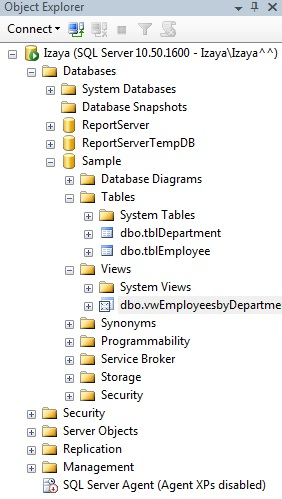
\includegraphics[width=0.5\textwidth]{CreateViewQuerySource}
    \caption{Project's Objects Explorer}
    \label{fig_21}
\end{figure}

As we can observe, we have 2 tables:
- tblDepartment (containing names of departments and their IDs)
- tblEmployee (containing all the information about the employees)
\\
Employee table will have 5 columns (ID, Name, Salary, Gender, DepartmentName)
and we will operate first of all by merging two tables, after this we will create a view. (note: by convention it is a good experience to start view names with vW)\\

\begin{figure}[ht!]
    \centering
    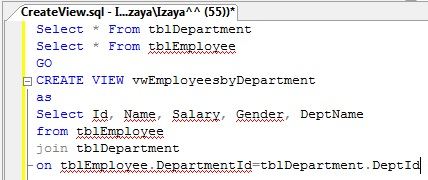
\includegraphics[width=0.5\textwidth]{CreateViewQuery}
    \caption{Creating View Query}
    \label{fig_21}
\end{figure}

Views simplify our work presenting the database for non-IT users, making it a lot more easier to generate, to manage accesses or to hide confidential data.
For our two tables, I will try to make different views for different kind of requests we'll get. \\
Let's give a specific table for someone who wants to join IT department and want to know his future co-workers:
\lstinputlisting[style=mystyle, language=SQL, caption={Views creating statements},]{sourcecode/PP_ITDep.sql}
So that's how the query will look like and the result will be this:
\begin{figure}[ht!]
    \centering
    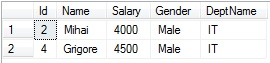
\includegraphics[width=0.5\textwidth]{ITDep}
    \caption{ITDepartment Query Result}
    \label{fig_21}
\end{figure}

In the Object Explorer we can see how we slowly add views in the Views Folder to the Sample Database that we are working in.
\begin{figure}[ht!]
    \centering
    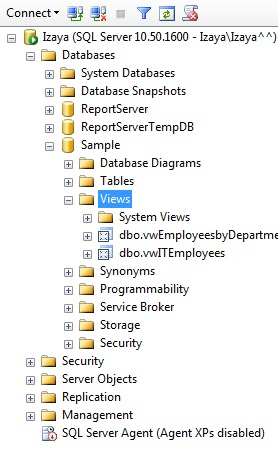
\includegraphics[width=0.5\textwidth]{ITDepSource}
    \caption{ITDepartment Query Result}
    \label{fig_21}
\end{figure}

Let's simulate the situation when we are publishing the database to all the employees or to third party. This is the case when some information from the table must be hide in order to protect status and behavior of the person.
For such a cases Views are a powerful tool that allows us to create a view from a table which will not contain the disturbing or personal information.
This is shown below:\\
\begin{figure}[ht!]
    \centering
    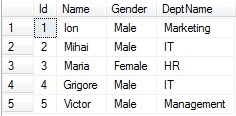
\includegraphics[width=0.5\textwidth]{NonConfidential}
    \caption{ITDepartment Query Result}
    \label{fig_21}
\end{figure}
As we can see, with a simple query I eliminated the column in which where the Salary of the employees by creating a view without this column, so the main table still holds this info, but for public eyes it is hiden.
\lstinputlisting[style=mystyle, language=SQL, caption={Views creating statements},]{sourcecode/PP_NonConfidential.sql}
\textbf{Update} for a view is done simply with clause Update and Set. In the following example I will change the name of a specific employee with a specific ID using Update clause. 
\begin{figure}[ht!]
    \centering
    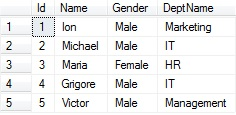
\includegraphics[width=0.5\textwidth]{Update}
    \caption{Updated View}
    \label{fig_21}
\end{figure}

Let's not forget that Views are also tables, and we can do things like deleting from a row or specific element, or to insert in a specific place our new data if it's free to insert.\\
\textbf{Deleting} a view is done by the command Drop, which performs in the following way:\\
\lstinputlisting[style=mystyle, language=SQL, caption={Views creating statements},]{sourcecode/Drop_viewCode.sql}
\begin{figure}[ht!]
    \centering
    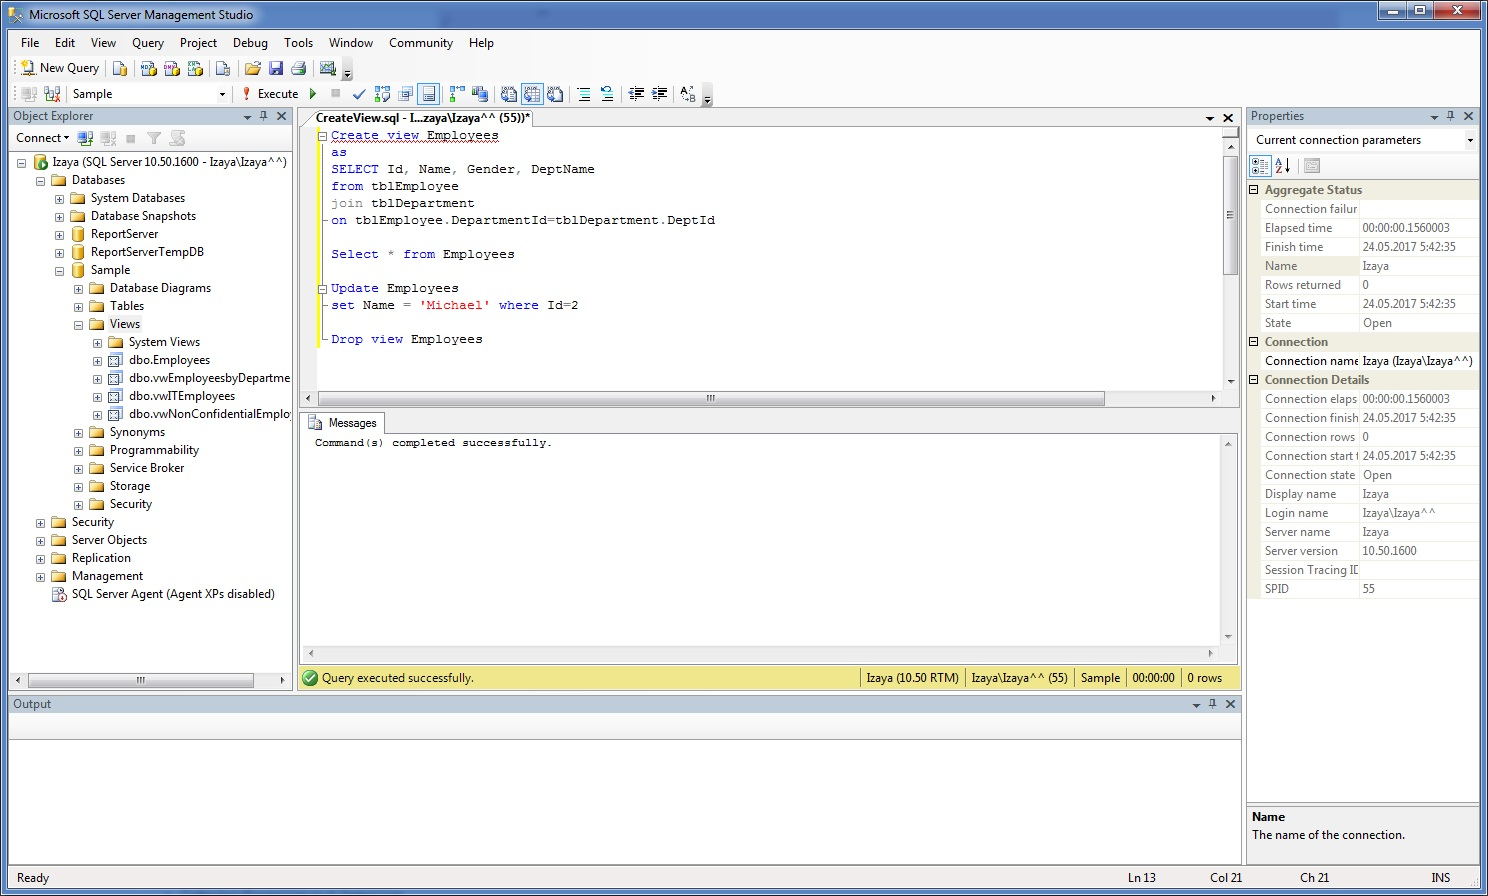
\includegraphics[width=0.5\textwidth]{DropView}
    \caption{Updated View}
    \label{fig_21}
\end{figure}

After we execute the DROP command we should see the elimination of the view in the Views folder of the project.\\
\begin{figure}[ht!]
    \centering
    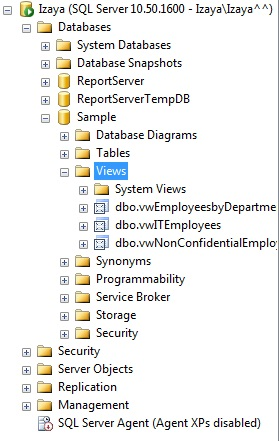
\includegraphics[width=0.5\textwidth]{DropViewAfter}
    \caption{Updated View}
    \label{fig_21}
\end{figure}

In such a simple way Views can facilitate work using simple query requests.
\clearpage